% !TEX root = ../notes.tex

% ================  (Interactive) Visualization ==============

\section{Data Visualization}
\subsection{Two main purposes}

In this chapter we are going to talk about visualization in general and then about what it is called interactive visualization. The first thing we do when we talk about visualization is to split it into two different tracks. 

\begin{itemize}
\item {The first one is about \emph{analysis}: you want to support reasoning about information. For instance, when you have a \texttt{DataFrame} you can make a plot of the distribution of the attribute in order to identify outliers, missing data and \emph{so forth}. In general with this kind of visualization you can do more like discover structures, quantify values and influences.
\textbf{This way of using visualization is extremely important for debugging purposes}.}

\item{The second  is the \emph{communication} part and it is about informing and persuade people.  The key difference in working in \emph{Data Science} and exclusively in \emph{Machine Learning} or \emph{Statistics} is the fact that you don't just stop after getting a good model and evaluating its accuracy. You would make a story that you convey to people.
For this reason we have to use visualization that can capture attention, can engage people and can tell a story visually (tell a story using visual tools takes a lot less time) and last but not least, you are focused only on certain aspects omitting others. It is a double-edged sword. That is because, on one hand you have to consider that there is an information overflow that people are suffering in general (we get too many media in which we consume information) so we do not want our visualization conveys more information than  a human being can actually get in a few seconds). On the other hand, we have to do it carefully, avoiding omitting some information just because difficult to handle or with, apparently, nonsense.}
\end{itemize}

\subsection{Data exploration}

In order to do a good \emph{Data exploration} analysis by means of visualization:

\begin{itemize}
\item {Get familiar with your favorite graphing package:}
\begin{itemize}
\item \texttt{Matplotlib} which is widely used in \texttt{Python}
\item \texttt{Seaborn} and \texttt{Bokeh} that are two additions on top of \texttt{Matplotlib}
\item \texttt{D3.js} (\texttt{Javascript}) is the most famous framework for interactive graphics
\end{itemize}
\item {Get fluent with plotting:}
\begin{itemize}
\item Histograms
\item Scatter plots
\item Line and bar plots
\end{itemize}
\end{itemize} 

\subsubsection{One variable}

Whenever we want to look at the data we can use histograms, they tell us a lot about the single variable. Once you plot them, you can try to figure out their distribution, for instance we can identify skewed distributions, multimodal or long tail data (Figure \ref{pic:long_tail}). 

\begin{figure}[H]%---------------FIG--------------
 \centering
 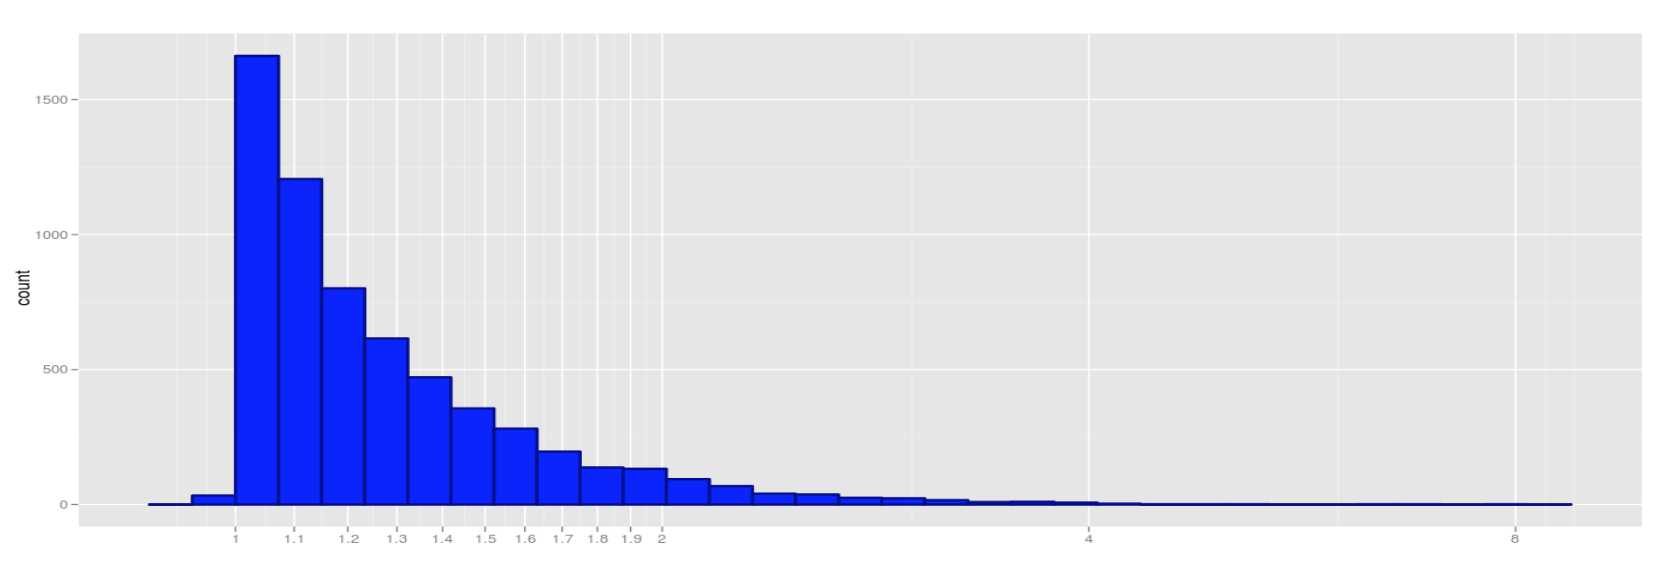
\includegraphics[width=13cm]{./img/06/long_tail}
 \caption{\label{pic:long_tail} Example of long tail data.}
\end{figure}

The latter is characterized by a bunch of bins that reveal a lot of occurrences and bars in the tail where we observe a very few occurrences. Many of this long tail data follow a \href{https://en.wikipedia.org/wiki/Power\_law\#Power-law\_probability\_distributions}{\emph{power-law}}. To claim the latter we need to run some test on data that proofs the statistical significance of our hypothesis, otherwise we can just state that it looks like a \emph{power-law}. For a graphical representation:

\begin{enumerate}
\item Sort the histogram counts by magnitude, descending.
\item Plot count vs bucket number on a log-log plot.
\end{enumerate}


\begin{figure}[H]%---------------FIG--------------
 \centering
 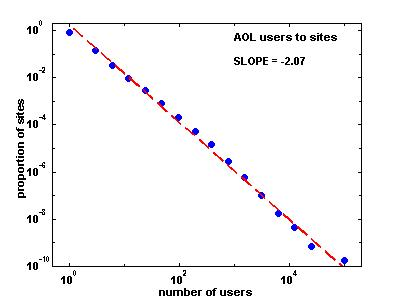
\includegraphics[width=10cm]{./img/06/power_law}
 \caption{\label{pic:power_law} Example \href{https://en.wikipedia.org/wiki/Zipf\%27s\_law}{power law}.}
\end{figure}


Generally this law is characteristic of social-influence processes, to know more look up for \emph{Preferential attachment}.

The \emph{multinomial} data registers more than one peak in the histogram, it suggests that there are two or more distinct populations of a sample. When you deal with something like this do not guess! Explore further by using, e.g., color and a histogram of multiple populations. 


\begin{figure}[H]%---------------FIG--------------
 \centering
 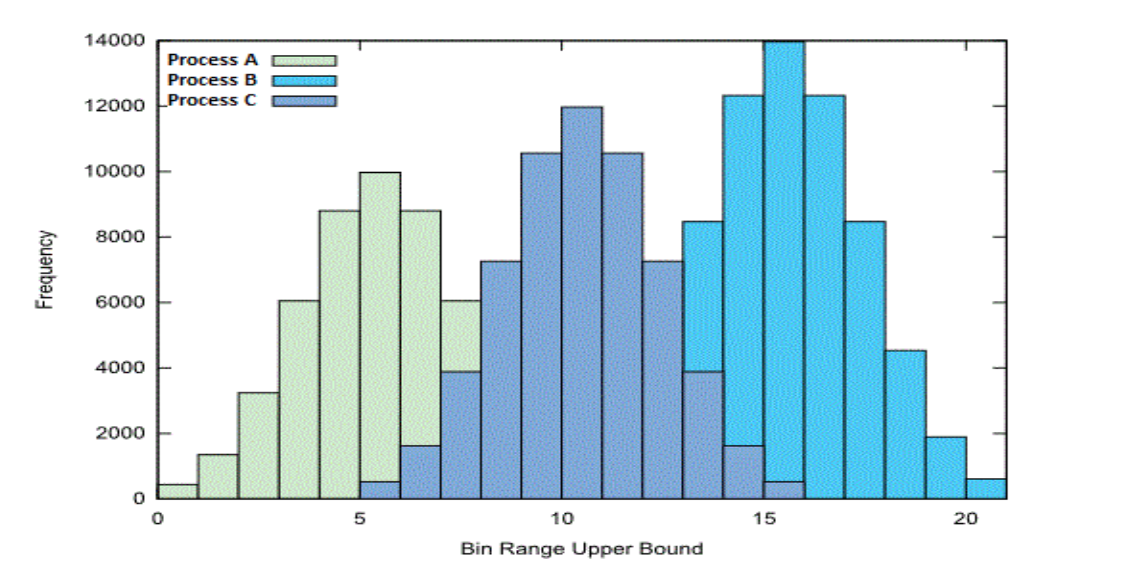
\includegraphics[width=13cm]{./img/06/multimodal}
 \caption{\label{pic:multimodal} Example of multimodal data.}
\end{figure}


Sometimes data is weird and is very hard to explain. Also in this case, do not guess! Trace through the data pipeline to find where the strangeness comes from. Usually it is a processing bug. Hence, check your code!

There is a way for a \emph{proactive Weird data Detection}. If data looks normal, take a picture and save it for later, then periodically compare new data with old whenever there is a pipeline update. Generally always try to have a theory of what the data should look like!

\subsubsection{More than one variable}
 
Most of the time we are interested in visualizing more than one variable, here a \emph{non-thorough} list of possibilities is listed:

\begin{itemize}
\item Two variables 
\begin{itemize}
\item \emph{Scatter plots} quickly expose the relationships between two variables
\end{itemize} 
\item  More than two variables
\begin{itemize}
\item \emph{Stacked plot}: stack variable is discrete, useful to explore data (Figure \ref{pic:stacked})
\begin{figure}[h]%---------------FIG--------------
 \centering
 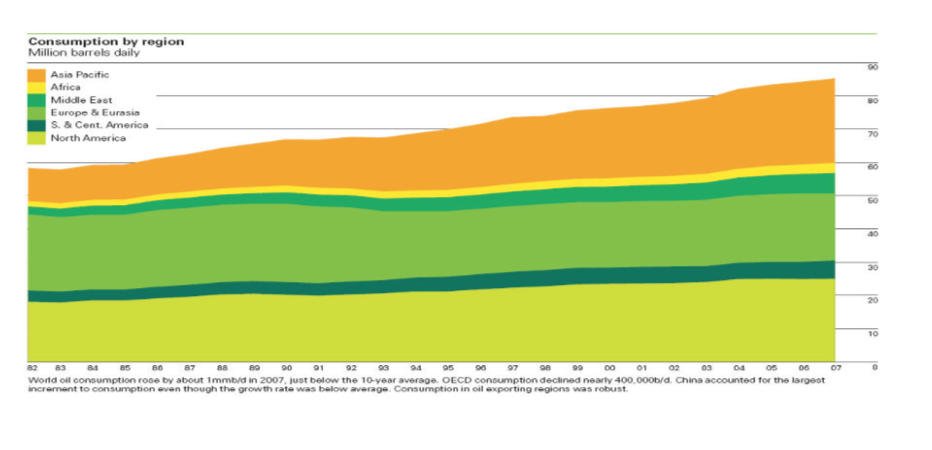
\includegraphics[width=13cm]{./img/06/stacked}
 \caption{\label{pic:stacked} Example of stacked plot.}
\end{figure}
\item \emph{Parallel coordinate plot}: one discrete variable, an arbitrary number of other variables (when this number increases it risks becoming very messy), see an example in Figure \ref{pic:parallel}
\begin{figure}[h]%---------------FIG--------------
 \centering
 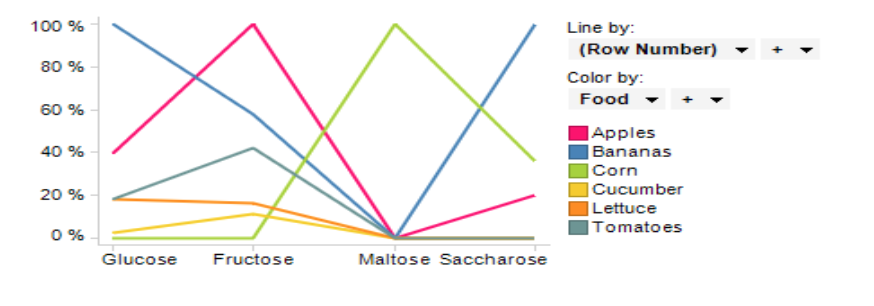
\includegraphics[width=13cm]{./img/06/parallel}
 \caption{\label{pic:parallel} Example of parallel plot.}
\end{figure}
\item \emph{Radar Chart}: one discrete variable (through the radar design), an arbitrary number of other variables (Figure \ref{pic:radar})
\begin{figure}[h]%---------------FIG--------------
 \centering
 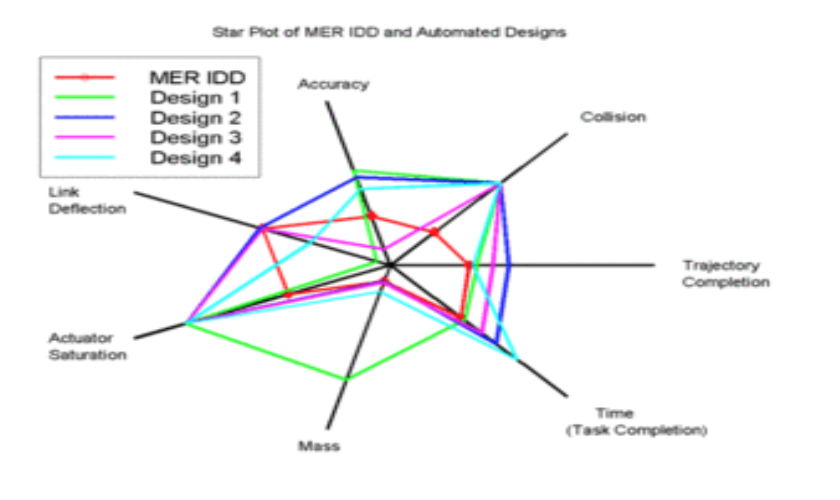
\includegraphics[width=13cm]{./img/06/radar}
 \caption{\label{pic:radar} Example of radar plot.}
\end{figure}
\end{itemize}
\end{itemize}


When you deal with a high number of variables, a valid idea to visualize in a better way is to reduce the number of variables applying algorithms, this pocess is called \emph{Dimensionality reduction}, one example is the \href{https://en.wikipedia.org/wiki/Principal\_component\_analysis}{ \emph{PCA}}. Intuitively, given twenty different variables, many tend to not variate a lot, \emph{PCA} extracts the couple of attributes that really make the difference allow visualization of high-dimensional continuous data in 2D using principal components. Hence, instead of directly plot multivariate data, try to think whether a dimensionality reduction can be useful.

We argued for analysts is important to form expectations of what the data should look like. This helps against pipeline errors and to identify interesting patterns. 
\\
But beware of seeing \href{https://en.wikipedia.org/wiki/Martian_canal}{\emph{Martian Canals}}: do not see things that are not there. Moreover, an observer should also be attuned to patterns that are not part of his theory, in other words, to expect the unexpected. 


\subsection{Moving Towards Interactive Viz}

Interactive visualization is a new field and it's getting more and more common. Our aim is to deliver results and this has been enabled by the new web technologies and in general by few frameworks essential for the current state of the art. \texttt{JavaScript} plays a very important role in the field. The vast majority of the libraries that allow to do visualization are in \href{https://www.codecademy.com/learn/javascript}{\texttt{JavaScript}}, so if you know how to use it or if you want to learn how to use it, it is definitely a good tool to have in your toolbar. 

A visualization is worth a thousand words! Representing in 2D more than two variables has been being a challenge since a long time ago. Even without the help of the machines, someone tried to do something in \href{https://en.wikipedia.org/wiki/Charles\_Joseph\_Minard}{this} field. Nowadays the technology allows the \emph{researchers} to go further and to use all their creativity and skills, nevertheless so many efforts should be put in. Lots of concepts have been developed and, for those interested, there are pioneers of the field that should be taken into \href{https://en.wikipedia.org/wiki/Edward\_Tufte}{consideration}.

As we already said the visualization has the characteristic of engaging the audience easily and it often results clear and understandable (be careful, not all the graphs and representations you look at are reliable, fair and proper!!). Hence it can be used to globally describe \href{https://www.ted.com/talks/hans\_rosling\_shows\_the\_best\_stats\_you\_ve\_ever\_seen}{phenomena} not easy to understand otherwise. Today, many are the \href{https://www.gapminder.org/tools/#\_chart-type=bubbles\&state\_time\_end=2015;\&entities\%2F\_minimap\_show\_geo.cat@=main\%2F\_religion\%2F\_2008;;;\&marker_color\_which=geo.main\%2F\_religion\%2F\_2008}{websites} where you can play with data using visualization.

Visualizing data is becoming a new way to spread information. More than ever, we recognize the existence of \emph{Data journalism}, more data are available, many people have programming skills. Thus, it is simple to find persons who combine both writing and programming skills. There are journals that stand out, such the \href{http://www.nytimes.com/interactive/2014/06/05/upshot/how-the-recession-reshaped-the-economy-in-255-charts.html?\_r=0}{\emph{New York Times}}, \emph{Forbes} and \emph{The Economist}. They build up teams of researchers who are the best experts in the field. Hence, they can be considered a great source of best practices in viz.

\subsection{Visualization definitions}

There is not a unique way to define visualization, here some definitions that try to include many few aspects are listed:

\begin{itemize}
\item \emph{Transformation of the symbolic into the geometric} (McCormick et al. 1987) 
\item \emph{... finding the artificial memory that best supports our natural means of perception.} (Bertin 1967)
\item \emph{The use of computer-generated, interactive, visual representations of data to amplify cognition.} (Card, Mackinlay \& Shneiderman 1999) 
\end{itemize}

\subsection*{The 10 rules}

When you do visualization you have to take care of the following \href{http://www.sealthreinhold.com/school/tuftes-rules/}{rules}:

\begin{enumerate}
\item \textbf{Show your data}: be careful of showing what you want to show, do not forget the main information;
\item \textbf{Use graphics}: glue together descriptions and figures;
\item \textbf{Avoid Chartjunk}: display your data in a fancy way, do not add anything that can make the interpretation harder;
\item \textbf{Utilize Data-ink} as much as you can, be careful when choosing what keep and remove;
\item \textbf{Use labels}: let the people understand what you are talking about;
\item \textbf{Utilize Micro/Macro}: an overview does not need so many details as when you zoom in;
\item \textbf{Separate Layers}: make more visible what you want the people to focus on;
\item \textbf{Use Multiples}: a thing different from the other captures the attention;
\item \textbf{Utilize Color} in a way such that data is interpreted;
\item \textbf{Understand Narrative}: when you tell a story respect time and space.
\end{enumerate}

\subsection*{Interactive chart design}

With interactive charts you can keep things very simple by hiding and dynamically revealing important structure.
On an interactive chart, you reveal the information most useful for navigating the chart. The aforementioned rules hold for the interactive charts as well.

\subsection*{The importance of magnitude}
\subsubsection*{Compare areas}

Let the reader compare areas is dangerous (Figure  \ref{pic:area}), avoid it whether possible or try to insert information to be able of making significant comparisons. Related to the capability of distinguishing and understanding magnitudes, in 1984, Cleveland and McGill wrote the paper
\href{https://www.cs.ubc.ca/\~tmm/courses/cpsc533c-04-spr/readings/cleveland.pdf}{\emph{Graphical Perception: Theory, Experimentation, and Application to the Development of Graphical Methods}} which identifies and analyzes a set of \emph{elementary perceptual tasks} conducted in the moment the reader extract quantitative information from graphs (Figure \ref{pic:magnitude}). 

\begin{figure}[H]%---------------FIG--------------
 \centering
 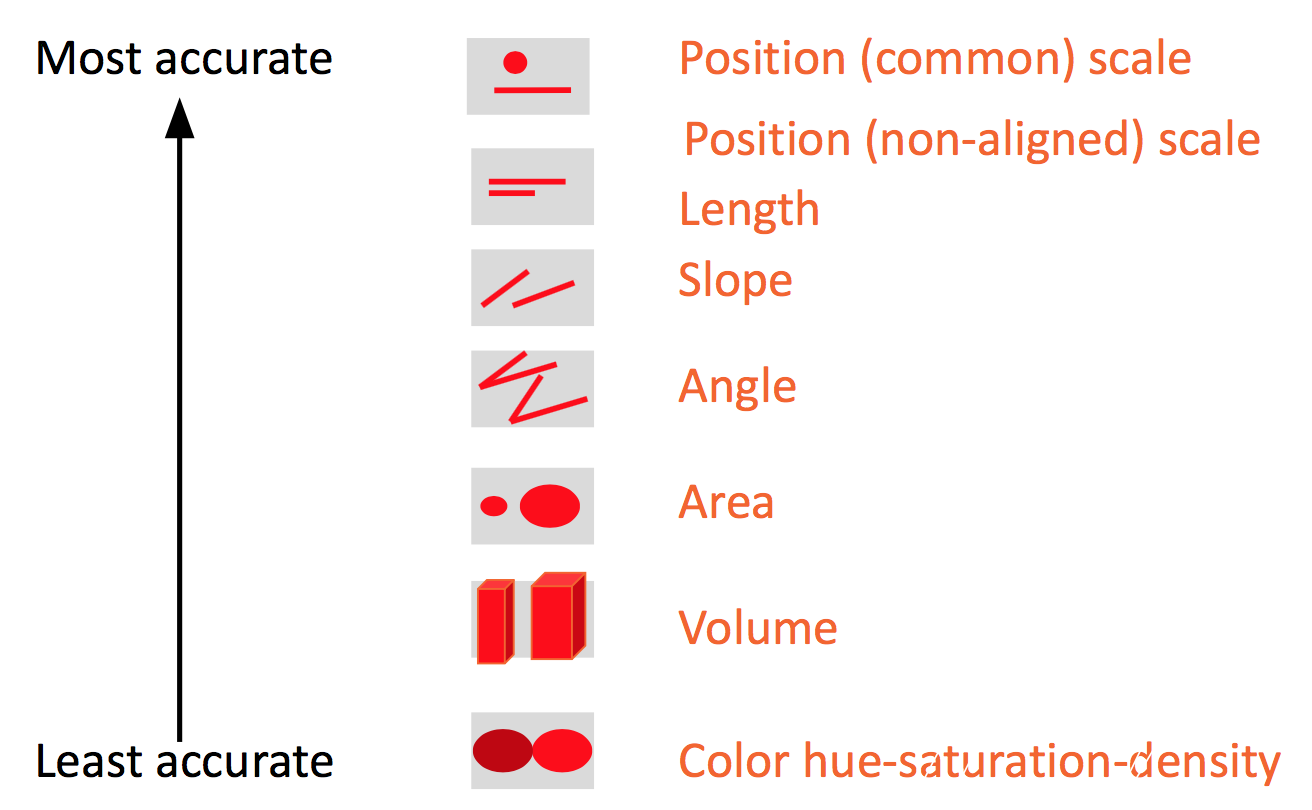
\includegraphics[width=13cm]{./img/06/magnitude}
 \caption{\label{pic:magnitude} What works and what does not.}
\end{figure}

\newpage
These tasks are sorted according to how accurately people perform them.

\begin{figure}[h]%---------------FIG--------------
 \centering
 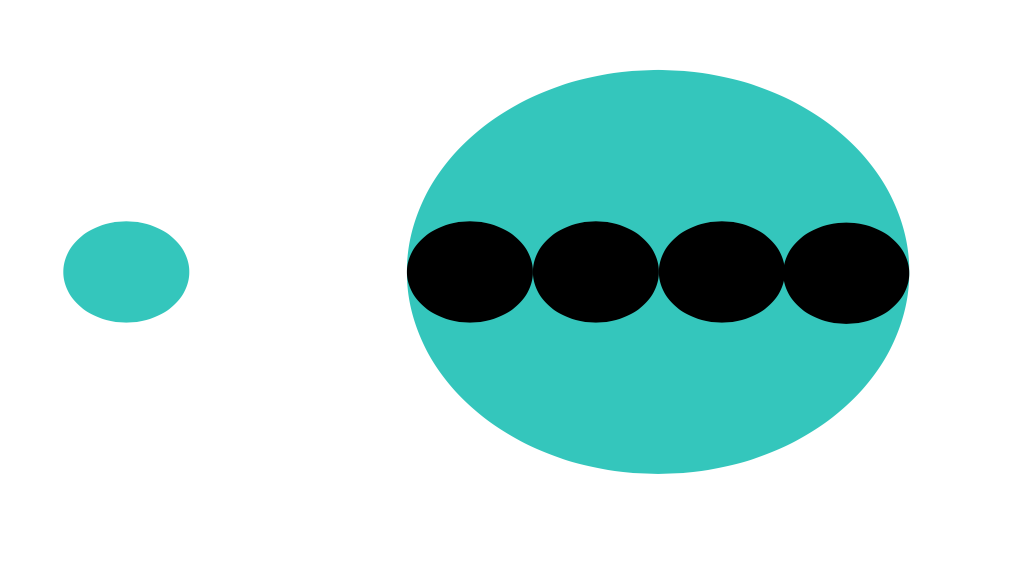
\includegraphics[width=12cm]{./img/06/area}
 \caption{\label{pic:area} How many times the \emph{little} one is included in the \emph{big} one? (Answer: 16)}
\end{figure}

\subsubsection*{Compare colors...}
Use a magnitude that allows people to easily read and interpret your data, noticeable differences are required. In 1846 the physicist Ernst Weber, defining \emph{I} as the intensity of the stimulus and \emph{S} the sensation, said that

$$\Delta S = k \frac{\Delta I}{I}.$$

It is known as the \emph{Weber's law} and reads out that a variation in the sensation is proportional to the magnitude of the original intensity of the stimulus. So as the base \emph{I} increase, we require a larger changes in  $\Delta I$ to notice the change. 

\subsubsection*{...And choose them}

Choose colors based on the information you want to convey:

\begin{itemize}
\item \emph{Sequential}: colors can be ordered from low to high (Figure \ref{pic:sequential})
\item \emph{Diverging}: two sequential schemes extended out from a critical midpoint value (Figure \ref{pic:diverging})
\item \emph{Categorical}: Lots of contrasts between each adjacent color (Figure \ref{pic:sequential})
\end{itemize}

\begin{figure}[H]%---------------FIG--------------
 \centering
 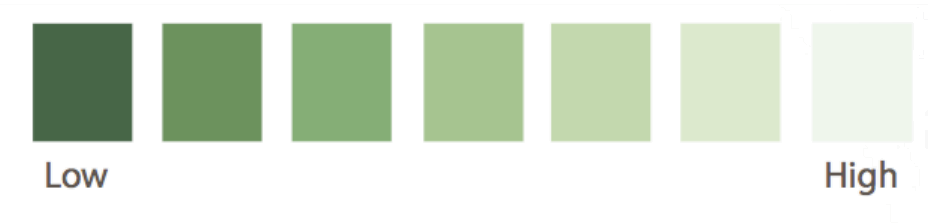
\includegraphics[width=13cm]{./img/06/sequential}
 \caption{\label{pic:sequential} Example of sequential colors.}
\end{figure}


\begin{figure}[H]%---------------FIG--------------
 \centering
 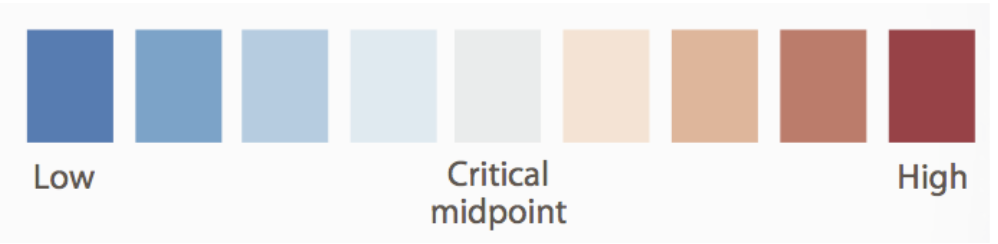
\includegraphics[width=13cm]{./img/06/diverging}
 \caption{\label{pic:diverging} Example of diverging colors.}
\end{figure}

\begin{figure}[H]%---------------FIG--------------
 \centering
 
\includegraphics[width=13cm]{./img/06/categorical}
 \caption{\label{pic:categorical} Example of categorical colors.}
\end{figure}

The usage of these tools depends on what you what to show. Anyway there are several \href{http://colorbrewer2.org/#type=sequential\&scheme=BuGn\&n=3}{online} sources that can help you to choose the color scheme according to your purpose.

\subsection*{Use Structure}

In 1912 Gestalt outlined principles that describe how our mind organizes individual visual elements into groups, to make sense of the entire visual. When designing a visual, these principles can be used to highlight patterns that are important to us, and downplay other patterns. The Figure  illustrates the \href{http://www.fusioncharts.com/blog/2014/03/how-to-use-the-gestalt-principles-for-visual-storytelling-podv/}{principles of Gestalt} which is relevant to visualization (Figure \ref{pic:gestalt}). Do not concentrate too much information, less is more!

\begin{figure}[H]%---------------FIG--------------
 \centering
 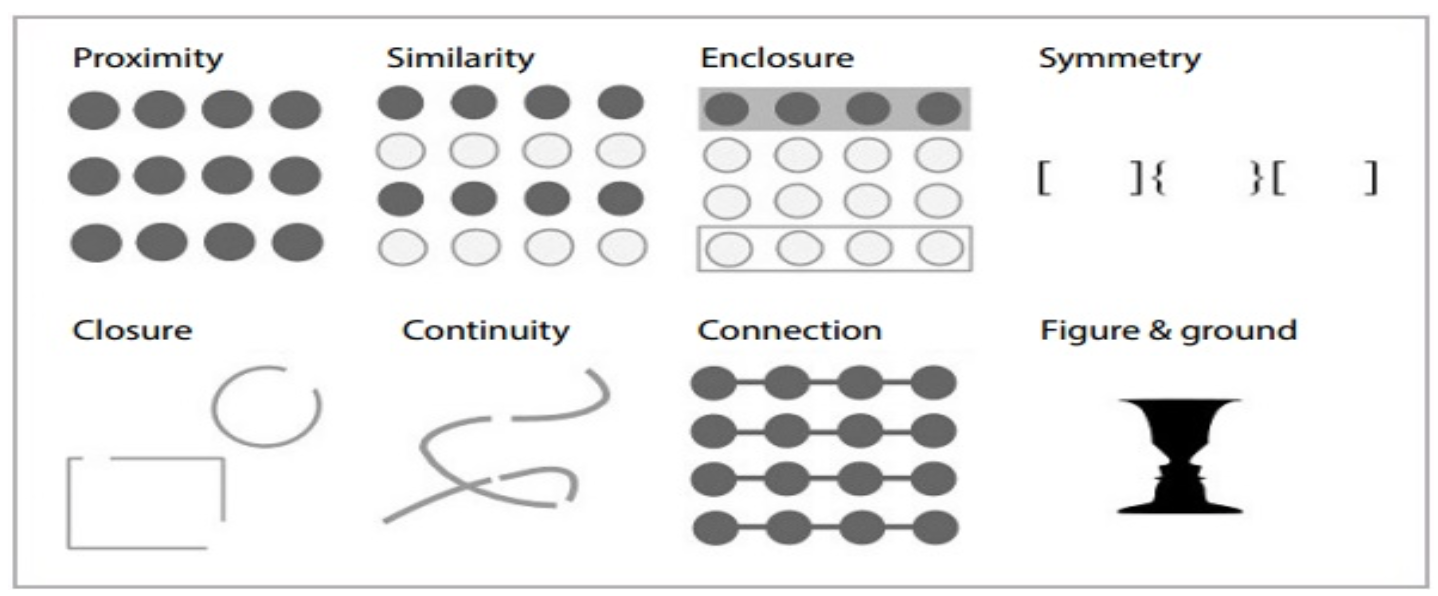
\includegraphics[width=13cm]{./img/06/gestalt}
 \caption{\label{pic:gestalt} Gestalt's principles.}
\end{figure}

Here is what we notice from each of the illustrations [\href{http://www.fusioncharts.com/blog/2014/03/how-to-use-the-gestalt-principles-for-visual-storytelling-podv/}{principles of Gestalt}]:

\begin{itemize}

\item \textbf{Proximity}: we see three rows of dots instead of four columns of dots because they are closer horizontally than vertically.
\item \textbf{Similarity}: we see similar-looking objects as part of the same group.
\item \textbf{Enclosure}: we group the first four and last four dots as two rows instead of eight dots.
\item \textbf{Symmetry}:we see three pairs of symmetrical brackets rather than six individual brackets.
\item \textbf{Closure}: we automatically close the square and circle instead of seeing three disconnected paths.
\item \textbf{Continuity}: we see one continuous path instead of three arbitrary ones.
\item \textbf{Connection}: we group the connected dots as belonging to the same group.
\item \textbf{Figure \& ground}: we either notice the two faces, or the vase. Whichever we notice becomes the figure, and the other the ground

\end{itemize}

These principles allow us to perform many tasks such as reduce the noise from charts, choose the ideal aspect ratio, and show relationships between elements more clearly. Let's look at a dashboard, and see these principles in action.

\subsection*{How to select the right chart}

The flowchart below can be helpful to understand the most suitable chart for your purpose.

\begin{figure}[H]%---------------FIG--------------
 \centering
 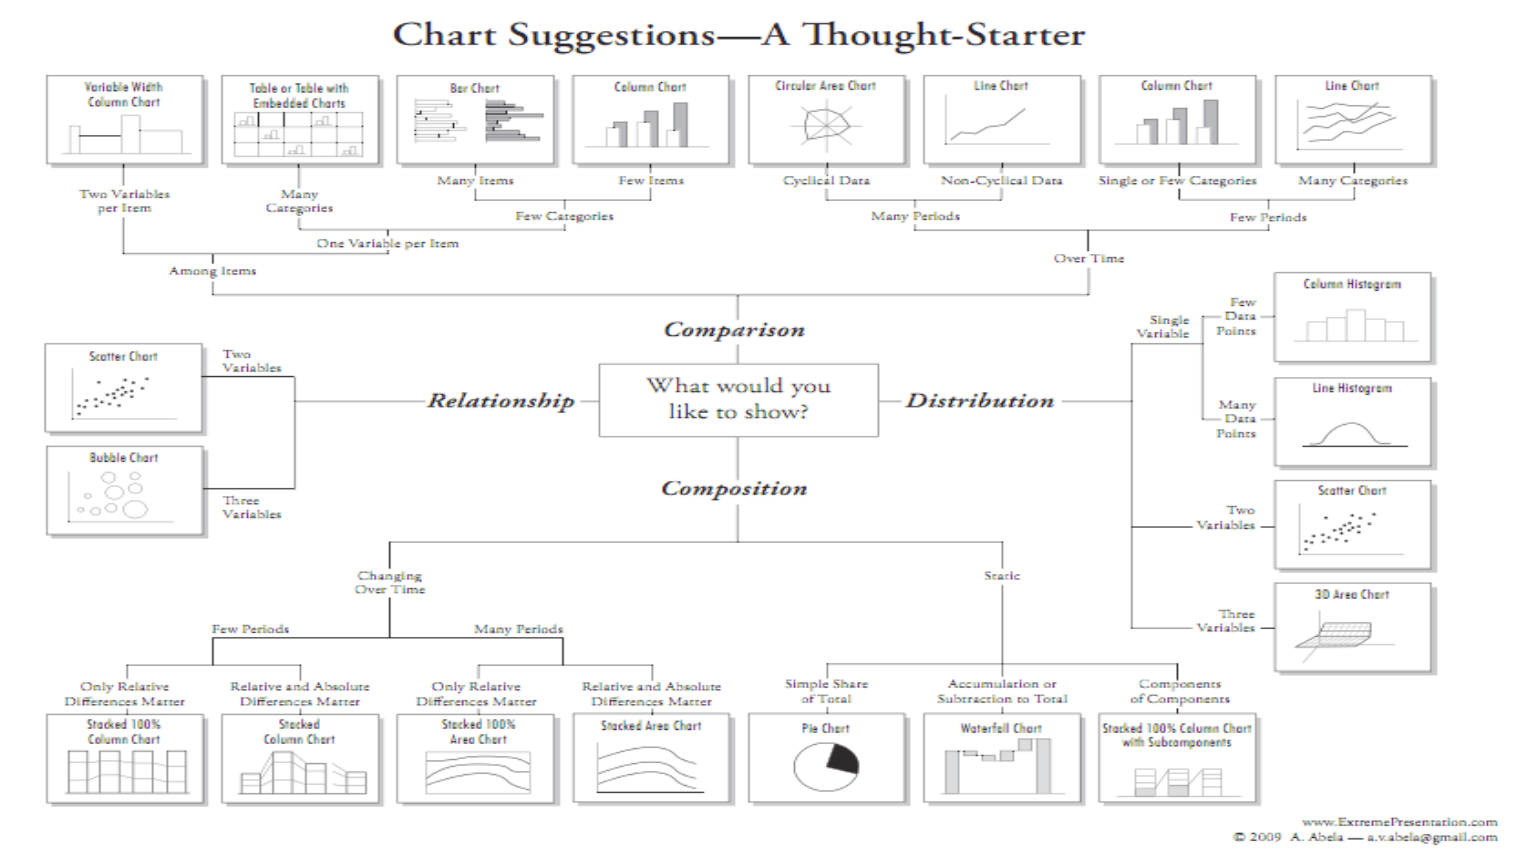
\includegraphics[width=16cm]{./img/06/flow_chart}
 \caption{\label{pic:flow_chart} Make your choice.}
\end{figure}

Instead of using the chart, you can also find sources, like \href{http://www.juiceanalytics.com}{\emph{Juice Analytics}}, that let you choose interactively, means some filters, the best chart according to your necessities.

\subsection{Interactive toolkits}

\begin{itemize}
\item \href{https://d3js.org}{\texttt{D3}} is, without doubt, the most widely used interactive visualization framework, developed around 2011 by Jeff Heer, Mike Bostock and Vadim Ogievetsky. \emph{Notes from the authors}: D3 is intentionally a low-level system. During the early design of D3, we even referred to it as a "visualization kernel" rather than a "toolkit" or "framework";

\item \href{https://vega.github.io/}{\texttt{Vega}} is a \emph{visualization grammar} developed on top of \texttt{d3.js}. It specifies graphics in \texttt{JSON} format;

\item \href{https://vega.github.io/vega/}{\texttt{Vincent}} is a Python-to-Vega translator;

\item \href{http://bokeh.pydata.org/en/latest/}{\texttt{Bokeh}} is an independent Viz library focused more heavily on big data visualization. Has both \texttt{Python} and \texttt{Scala} bindings; 

\end{itemize}
